\chapter{计数器考试变式题}

\section*{题目1：模7计数器}

\textbf{题目}：设计一个模7计数器（0-6循环），写出VHDL代码和Testbench。

\textbf{分析}：
\begin{itemize}
  \item $N=7$，$k=\lceil\log_2 7\rceil = 3$位
  \item 清零条件：cnt = 6(110)
  \item 状态序列：000→001→010→011→100→101→110→000
\end{itemize}

\textbf{VHDL}：
\begin{lstlisting}
signal cnt : std_logic_vector(2 downto 0);
process(clk, rst_n)
begin
  if rst_n = '0' then cnt <= "000";
  elsif rising_edge(clk) then
    if cnt = "110" then cnt <= "000";
    else cnt <= cnt + 1; end if;
  end if;
end process;
\end{lstlisting}

\section*{题目2：模13计数器}

\textbf{题目}：设计模13计数器（0-12循环），写出VHDL。

\textbf{分析}：
\begin{itemize}
  \item $N=13$，$k=\lceil\log_2 13\rceil = 4$位
  \item 清零：cnt = 12(1100)
\end{itemize}

\textbf{VHDL}：
\begin{lstlisting}
signal cnt : std_logic_vector(3 downto 0);  -- 4位
 if cnt = "1100" then cnt <= "0000";  -- =12清零
else cnt <= cnt + 1;
\end{lstlisting}

\section*{题目3：模3计数器}

\textbf{题目}：设计模3计数器，画出状态转移图，写VHDL。

\textbf{分析}：
\begin{itemize}
  \item $N=3$，$k=2$位
  \item 状态：00→01→10→00
  \item 清零：cnt=2(10)
\end{itemize}

\textbf{状态图}：
\begin{center}
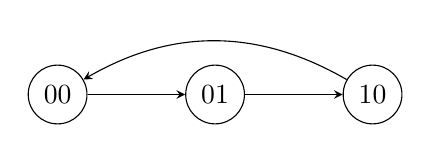
\begin{tikzpicture}[->, >=stealth]
  \node[draw,circle] (s0) at (0,0) {00};
  \node[draw,circle] (s1) at (2,0) {01};
  \node[draw,circle] (s2) at (4,0) {10};
  \draw (s0) -- (s1);
  \draw (s1) -- (s2);
  \draw (s2) edge[bend right] (s0);
\end{tikzpicture}
\end{center}

\section*{题目4：带使能的模8计数器}

\textbf{题目}：设计带使能信号en的模8计数器。en=1时计数，en=0时保持。

\textbf{VHDL}：
\begin{lstlisting}
 if rising_edge(clk) then
  if en = '1' then
    cnt <= cnt + 1;  -- 3位自然溢出=模8
  end if;
end if;
\end{lstlisting}

\section*{题目5：带同步加载的模10计数器}

\textbf{题目}：设计带同步加载（load）的模10计数器。load=1时cnt = data\_in；load=0时正常计数（0-9）。

\textbf{VHDL}：
\begin{lstlisting}
 if rising_edge(clk) then
  if load = '1' then
    cnt <= data_in;
  elsif cnt = "1001" then
    cnt <= "0000";
  else
    cnt <= cnt + 1;
  end if;
end if;
\end{lstlisting}

\section*{题目6：递增/递减双向计数器}

\textbf{题目}：设计模16双向计数器。up=1递增，up=0递减。

\textbf{VHDL}：
\begin{lstlisting}
 if rising_edge(clk) then
  if up = '1' then
    cnt <= cnt + 1;
  else
    cnt <= cnt - 1;
  end if;
end if;
\end{lstlisting}

\section*{题目7：模10 BCD计数器带7段显示}

\textbf{题目}：设计模10 BCD计数器 + BCD-7段译码器。输出驱动7段数码管显示0-9。

\section*{题目8：模60计数器（秒/分计数器）}

\textbf{题目}：设计模60计数器用于时钟应用。输出秒/分的十位和个位。

\textbf{分析}：见第三部分第八章BCD模60计数器。

\section*{题目9：模24 BCD计数器}

\textbf{题目}：设计模24 BCD计数器。0-23循环。

\textbf{分析}：十位模3（0-2），个位模10（0-9）。清零条件：23。

\section*{题目10：模100 BCD计数器}

\textbf{题目}：设计两位BCD模100计数器（00-99循环）。

\textbf{分析}：个位每满10向十位进位。十位满9+个位满9（即99）时清零。

\section*{题目11：给定计数器时序图，推断模值}

\textbf{题目}：观察计数器Q2Q1Q0的波形：000→001→010→011→100→000→...。求模值。

\textbf{解}：出现了5个不同状态（000-100），所以模值=5。

\section*{题目12：给定VHDL推断模值}

\textbf{题目}：
\begin{lstlisting}
 if cnt = "1010" then cnt <= "0000";
else cnt <= cnt + 1;
\end{lstlisting}
求模值N。

\textbf{解}：清零条件是cnt=10(1010)，所以N=10+1=11？不对！
清零条件=cnt=1010=10，此时cnt还未计数到11就被清零了。
模值=清零条件值+1=10+1=11？再确认：cnt从0计到10清零，所以N=11。

\textbf{关键公式}：模值 = 清零比较值 + 1

\section*{题目13：分析计数器最大工作频率}

\textbf{题目}：4位行波进位加法器的进位链延迟为每个FA=2ns，D触发器$t_{setup}=1$ns，$t_{cko}=1$ns。求计数器的最大工作频率。

\textbf{分析}：
关键路径延迟 = $t_{cko}$ + 进位链延迟(4×2=8ns) + $t_{setup}$ = 1+8+1 = 10ns
$f_{max} = 1/10\text{ns} = 100\text{MHz}$

\section*{题目14：多个计数器级联的分析}

\textbf{题目}：模8计数器 + 模5计数器级联。总模值是多少？

\textbf{解}：模8每8拍产生一次进位，模5每收到进位+1。
总模值 = 8×5 = 40。

\textbf{通用公式}：级联总模值 = $M_1 \times M_2 \times \dots \times M_k$

\section*{题目15：BCD计数器的非法状态恢复}

\textbf{题目}：模10 BCD计数器可能因干扰进入非法状态(1010-1111)。设计自恢复逻辑。

\textbf{解}：
\begin{lstlisting}
 if cnt >= "1010" then  -- 非法状态
  cnt <= "0000";
elsif cnt = "1001" then
  cnt <= "0000";
else
  cnt <= cnt + 1;
end if;
\end{lstlisting}

\section*{题目16-20：综合应用题}

\subsection*{题目16：数字钟核心}
设计时分秒计数器（模60秒+模60分+模24时）。

\subsection*{题目17：带暂停的计数器}
Pause=1时暂停计数，pause=0时恢复。

\subsection*{题目18：带预置位的倒计时计数器}
从预置值倒计时到0，到0后重新加载预置值。

\subsection*{题目19：两相正交计数器}
输出两个相位差90度的方波（格雷码计数器的一种应用）。

\subsection*{题目20：用计数器实现序列检测}
计数器状态作为地址，ROM存放序列，输出+检测逻辑。

\begin{examtip}[计数器类题目的统一解法]
\textbf{第一步：}确定模值N
\textbf{第二步：}$k = \lceil \log_2 N \rceil$，确定位宽
\textbf{第三步：}清零条件 = N-1 的二进制
\textbf{第四步：}写VHDL模板（if cnt=N-1 then cnt<=0 else cnt<=cnt+1）
\textbf{第五步：}如果有级联，低位进位接高位时钟使能

\textbf{关键公式}：
\begin{itemize}
  \item 模值 = 清零比较值 + 1
  \item 总模值（级联）= $M_1 \times M_2$
  \item $2^N$模值不需要显式清零
\end{itemize}
\end{examtip}
